
%🍁%
%🍁% \chapter{Fruitful functions  |  有返回值的函数}
\chapter{有返回值的函数}
\label{fruitchap}

%🍁% Many of the Python functions we have used, such as the math
%🍁% functions, produce return values.  But the functions we've written
%🍁% are all void: they have an effect, like printing a value
%🍁% or moving a turtle, but they don't have a return value.  In
%🍁% this chapter you will learn to write fruitful functions.

许多我们前面使用过的 Python 函数都会产生返回值, 如数学函数。
但目前我们所写的函数都是空函数 (void): 它们产生某种效果, 像打印一个值或是移动乌龟,但是并没有返回值。
在本章中, 你将学习如何写一个有返回值的函数。

%🍁% \section{Return values  |  返回值}
\section{返回值}
\index{return value}  \index{返回值}

%🍁% Calling the function generates a return
%🍁% value, which we usually assign to a variable or use as part of an
%🍁% expression.

调用一个有返回值的函数会生成一个返回值, 我们通常将其赋值给某个变量或是作为表达式的一部分。

\begin{lstlisting}
e = math.exp(1.0)
height = radius * math.sin(radians)
\end{lstlisting}

%
%🍁% The functions we have written so far are void.  Speaking casually,
%🍁% they have no return value; more precisely,
%🍁% their return value is {\tt None}.

目前我们所写的函数都是空函数。
泛泛地来看, 它们没有返回值; 更准确地说, 它们的返回值是 \li{None} 。

%🍁% In this chapter, we are (finally) going to write fruitful functions.
%🍁% The first example is {\tt area}, which returns the area of a circle
%🍁% with the given radius:

本章中, 我们(终于)要开始写有返回值的函数了。
第一个例子是 \li{area} , 返回给定半径圆的面积。

\begin{lstlisting}
def area(radius):
    a = math.pi * radius**2
    return a
\end{lstlisting}

%
%🍁% We have seen the {\tt return} statement before, but in a fruitful
%🍁% function the {\tt return} statement includes
%🍁% an expression.  This statement means: ``Return immediately from
%🍁% this function and use the following expression as a return value.''
%🍁% The expression can be arbitrarily complicated, so we could
%🍁% have written this function more concisely:

我们之前已经见过 \li{return} 语句,但在有返回值的函数中, \li{return} 语句包含一个表达式。
条语句的意思是:``马上从该函数返回,并使用接下来的表达式作为返回值。''
此表达式可以是任意复杂的, 因此我们可以将该函数写得更简洁些:
\index{return statement}  \index{statement!return}

\begin{lstlisting}
def area(radius):
    return math.pi * radius**2
\end{lstlisting}

%
%🍁% On the other hand, {\bf temporary variables} like {\tt a} can make
%🍁% debugging easier.

另一方面, 像 \li{a} 这样的 {\em 临时变量} (temporary variables) 能使调试变得更简单。

\index{temporary variable}  \index{variable!temporary}

%🍁% Sometimes it is useful to have multiple return statements, one in each
%🍁% branch of a conditional:

有时,在条件语句的每一个分支内各有一个返回语句会很有用:

\begin{lstlisting}
def absolute_value(x):
    if x < 0:
        return -x
    else:
        return x
\end{lstlisting}

%
%🍁% Since these {\tt return} statements are in an alternative conditional,
%🍁% only one runs.

因为这些 \li{return} 语句在不同的条件内,最后只有{\bf 一个}会被执行。

%🍁% As soon as a return statement runs, the function
%🍁% terminates without executing any subsequent statements.
%🍁% Code that appears after a {\tt return} statement, or any other place
%🍁% the flow of execution can never reach, is called {\bf dead code}.

一旦一条返回语句执行,函数则终止,不再执行后续的语句。出现在某条return语句之后的代码,或者在执行流程永远不会到达之处的代码,被称为 {\em 死代码} (dead code)。
\index{dead code}  \index{死代码}

%🍁% In a fruitful function, it is a good idea to ensure
%🍁% that every possible path through the program hits a
%🍁% {\tt return} statement.  For example:

在一个有返回值的函数中, 最好保证程序执行的每一个流程最终都会碰到一个 \li{return} 语句。例如:

\begin{lstlisting}
def absolute_value(x):
    if x < 0:
        return -x
    if x > 0:
        return x
\end{lstlisting}

%
%🍁% This function is incorrect because if {\tt x} happens to be 0,
%🍁% neither condition is true, and the function ends without hitting a
%🍁% {\tt return} statement.  If the flow of execution gets to the end
%🍁% of a function, the return value is {\tt None}, which is not
%🍁% the absolute value of 0.

这个函数是有问题的。 原因是如果 \li{x} 恰好是 0, 则没有条件为真, 函数将会在未执行任何 \li{return} 语句的情况下终止。 如果函数按照这种执行流程执行完毕,返回值将是 \li{None} ,这可不是 0 的绝对值。
\index{None special value}  \index{special value!None}

\begin{lstlisting}
>>> absolute_value(0)
None
\end{lstlisting}

%
%🍁% By the way, Python provides a built-in function called
%🍁% {\tt abs} that computes absolute values.

顺便说一下,Python提供了一个的内建函数 \li{abs} 用来计算绝对值。
\index{abs function}  \index{function!abs}

%🍁% As an exercise, write a {\tt compare} function
%🍁% takes two values, {\tt x} and {\tt y}, and returns {\tt 1} if {\tt x > y},
%🍁% {\tt 0} if {\tt x == y}, and {\tt -1} if {\tt x < y}.

我们来做个练习,写一个比较函数 \li{compare} ,接受两个值 \li{x} 和 \li{y} 。
如果 \li{x > y}, 则返回 \li{1} ;如果 \li{x == y}, 则返回 \li{0} ;如果 \li{x < y},则返回 \li{-1} 。
\index{compare function}  \index{function!compare}


%🍁% \section{Incremental development  |  增量式开发}
\section{增量式开发}
\label{incremental.development}
\index{development plan!incremental}  \index{开发计划!增量式}

%🍁% As you write larger functions, you might find yourself
%🍁% spending more time debugging.

随着你写的函数越来越大,你在调试上花的时候可能会越来越多。

%🍁% To deal with increasingly complex programs,
%🍁% you might want to try a process called
%🍁% {\bf incremental development}.  The goal of incremental development
%🍁% is to avoid long debugging sessions by adding and testing only
%🍁% a small amount of code at a time.

为了应对越来越复杂的程序,你可以开始尝试叫作 {\em 增量式开发} (incremental development) 的方法。 增量式开发的目标,是通过每次只增加和测试少量代码,来避免长时间的调试。
\index{testing!incremental development}  \index{Pythagorean theorem}
\index{测试!增量开发}

%🍁% As an example, suppose you want to find the distance between two
%🍁% points, given by the coordinates $(x_1, y_1)$ and $(x_2, y_2)$.
%🍁% By the Pythagorean theorem, the distance is:

举个例子,假设你想计算两个给定坐标点 $(x_1, y_1)$ 和 $(x_2, y_2)$ 之间的距离。根据毕达哥拉斯定理\footnote{译注:the Pythagorean theorem, 即勾股定理},二者的距离是:


\begin{displaymath}
\mathrm{distance} = \sqrt{(x_2 - x_1)^2 + (y_2 - y_1)^2}
\end{displaymath}

%
%🍁% The first step is to consider what a {\tt distance} function should
%🍁% look like in Python.  In other words, what are the inputs (parameters)
%🍁% and what is the output (return value)?

第一步要考虑的是在 Python 中,距离函数看起来会是什么样。换句话说,输入(形参)和输出(返回值)是什么?

%🍁% In this case, the inputs are two points, which you can represent
%🍁% using four numbers.  The return value is the distance represented by
%🍁% a floating-point value.

本例中,输入是可以用 4 个数表示的两个点。 返回值是距离, 用浮点数表示。

%🍁% Immediately you can write an outline of the function:

现在你就可以写出此函数的轮廓了:

\begin{lstlisting}
def distance(x1, y1, x2, y2):
    return 0.0
\end{lstlisting}

%
%🍁% Obviously, this version doesn't compute distances; it always returns
%🍁% zero.  But it is syntactically correct, and it runs, which means that
%🍁% you can test it before you make it more complicated.

显然,此版本不能计算距离;它总是返回 0 。但是在语法上它是正确的,并且能运行,这意味着你可以在使它变得更复杂之前测试它。

%🍁% To test the new function, call it with sample arguments:

用样例实参调用它来进行测试。

\begin{lstlisting}
>>> distance(1, 2, 4, 6)
0.0
\end{lstlisting}

%
%🍁% I chose these values so that the horizontal distance is 3 and the
%🍁% vertical distance is 4; that way, the result is 5, the hypotenuse
%🍁% of a 3-4-5 triangle. When testing a function, it is
%🍁% useful to know the right answer.

我选择的这些值,可以使水平距离为 3 ,垂直距离为 4 ;
这样结果自然是 5,构成了一个勾三股四弦五的直角三角形。
测试一个函数时,知道正确的答案是很有用的。
\index{testing!knowing the answer}
\index{测试!已知结果}

%🍁% At this point we have confirmed that the function is syntactically
%🍁% correct, and we can start adding code to the body.
%🍁% A reasonable next step is to find the differences
%🍁% $x_2 - x_1$ and $y_2 - y_1$.  The next version stores those values in
%🍁% temporary variables and prints them.

此时我们已经确认这个函数在语法上是正确的,我们可以开始往函数体中增加代码。
下一步合理的操作,应该是求 $x_2 - x_1$ 和 $y_2 - y_1$ 这两个差值。
下一个版本在临时变量中存储这些值并打印出来。

\begin{lstlisting}
def distance(x1, y1, x2, y2):
    dx = x2 - x1
    dy = y2 - y1
    print('dx is', dx)
    print('dy is', dy)
    return 0.0
\end{lstlisting}

%
%🍁% If the function is working, it should display \verb"dx is 3" and
%🍁% \verb"dy is 4".  If so, we know that the function is getting the right
%🍁% arguments and performing the first computation correctly.  If not,
%🍁% there are only a few lines to check.

如果这个函数正常运行,它应该显示 \li{dx is 3}  以及 \li{dy is 4} 。
这样的话我们就知道函数获得了正确的实参并且正确执行了第一步计算。
如果不是,也只要检查几行代码。

%🍁% Next we compute the sum of squares of {\tt dx} and {\tt dy}:

下一步我们计算 \li{dx} 和 \li{dy} 的平方和。

\begin{lstlisting}
def distance(x1, y1, x2, y2):
    dx = x2 - x1
    dy = y2 - y1
    dsquared = dx**2 + dy**2
    print('dsquared is: ', dsquared)
    return 0.0
\end{lstlisting}

%
%🍁% Again, you would run the program at this stage and check the output
%🍁% (which should be 25).
%🍁% Finally, you can use {\tt math.sqrt} to compute and return the result:

再一次运行程序并检查结果 (应该是 25 )。
最后,你可以使用 \li{math.sqrt} 计算并返回结果。
\index{sqrt}  \index{function!sqrt}

\begin{lstlisting}
def distance(x1, y1, x2, y2):
    dx = x2 - x1
    dy = y2 - y1
    dsquared = dx**2 + dy**2
    result = math.sqrt(dsquared)
    return result
\end{lstlisting}

%
%🍁% If that works correctly, you are done.  Otherwise, you might
%🍁% want to print the value of {\tt result} before the return
%🍁% statement.

如果其正确运行的话,你就成功了。否则你可能想在 \li{return} 语句前打印结果检查一下。

%🍁% The final version of the function doesn't display anything when it
%🍁% runs; it only returns a value.  The {\tt print} statements we wrote
%🍁% are useful for debugging, but once you get the function working, you
%🍁% should remove them.  Code like that is called {\bf scaffolding}
%🍁% because it is helpful for building the program but is not part of the
%🍁% final product.

该函数的最终版不会在运行时显示任何东西,仅仅返回一个值。
我们之前写的 \li{print} 语句在调试时是很有用的, 不过在函数能够正确运行之后, 你就该删了它们。
我们称这样的代码为 {\em 脚手架代码} (scaffolding) , 因为它对程序的构建很有用, 但不是最终产品的一部分。
\index{scaffolding}

%🍁% When you start out, you should add only a line or two of code at a
%🍁% time.  As you gain more experience, you might find yourself writing
%🍁% and debugging bigger chunks.  Either way, incremental development
%🍁% can save you a lot of debugging time.

当你刚开始的时候, 最好每次只加入一两行代码。
随着经验见长, 你会发现自己可以编写、调试更大的代码块了。
无论哪种方式, 增量式开发都能节省你大量的调试时间。

%🍁% The key aspects of the process are:

这种开发方式的关键是:


%🍁% \begin{enumerate}
%🍁% \item Start with a working program and make small incremental changes.
%🍁% At any point, if there is an error, you should have a good idea
%🍁% where it is.
%🍁%
%🍁% \item Use variables to hold intermediate values so you can
%🍁% display and check them.
%🍁%
%🍁% \item Once the program is working, you might want to remove some of
%🍁% the scaffolding or consolidate multiple statements into compound
%🍁% expressions, but only if it does not make the program difficult to
%🍁% read.
%🍁% \end{enumerate}

\begin{enumerate}
\item 从一个能运行的程序开始,并且每次只增加少量改动。无论你何时遇到错误,都能够清楚定位错误的源头。

\item 用临时变量存储中间值,这样你就能显示并检查它们。

\item 一旦程序正确运行,你要删除一些脚手架代码,或者将多条语句组成复合表达式,但是前提是不会影响程序的可读性。
\end{enumerate}

%🍁% As an exercise, use incremental development to write a function
%🍁% called {\tt hypotenuse} that returns the length of the hypotenuse of a
%🍁% right triangle given the lengths of the other two legs as arguments.
%🍁% Record each stage of the development process as you go.

我们来做个练习:运用增量开发方式,写一个叫作 \li{hypotenuse} 的函数,接受直角三角形的两直角边长作为实参,返回该三角形斜边的长度。记录下你开发过程中的每一步。
\index{hypotenuse}



%🍁% \section{Composition  |  组合}
\section{组合}
\index{composition}  \index{function composition}

%🍁% As you should expect by now, you can call one function from within
%🍁% another.  As an example, we'll write a function that takes two points,
%🍁% the center of the circle and a point on the perimeter, and computes
%🍁% the area of the circle.

你现在应该已经猜到了,你可以从一个函数内部调用另一个函数。
作为示例,我们接下来写一个函数,接受两个点为参数,分别是圆心和圆周上一点,然后计算圆的面积。

%🍁% Assume that the center point is stored in the variables {\tt xc} and
%🍁% {\tt yc}, and the perimeter point is in {\tt xp} and {\tt yp}. The
%🍁% first step is to find the radius of the circle, which is the distance
%🍁% between the two points.  We just wrote a function, {\tt
%🍁% distance}, that does that:

假设圆心坐标存储在变量 \li{xc} 和 \li{yc} 中,圆周上的点的坐标存储在 \li{xp} 和 \li{yp} 中。第一步是计算圆半径,也就是这两个点的距离。
我们刚写的 \li{distance} 函数就可以计算距离:

\begin{lstlisting}
radius = distance(xc, yc, xp, yp)
\end{lstlisting}

%
%🍁% The next step is to find the area of a circle with that radius;
%🍁% we just wrote that, too:

下一步是用得到的半径计算圆面积;我们也刚写了这样的函数:

\begin{lstlisting}
result = area(radius)
\end{lstlisting}

%
%🍁% Encapsulating these steps in a function, we get:

将这些步骤封装在一个函数中,可以得到下面的函数:
\index{encapsulation}  \index{封装}

\begin{lstlisting}
def circle_area(xc, yc, xp, yp):
    radius = distance(xc, yc, xp, yp)
    result = area(radius)
    return result
\end{lstlisting}

%
%🍁% The temporary variables {\tt radius} and {\tt result} are useful for
%🍁% development and debugging, but once the program is working, we can
%🍁% make it more concise by composing the function calls:

临时变量 \li{radius} 和 \li{result} 对于开发调试很有用的,但是
一旦函数正确运行了,我们可以通过合并函数调用,将程序变得更简洁:

\begin{lstlisting}
def circle_area(xc, yc, xp, yp):
    return area(distance(xc, yc, xp, yp))
\end{lstlisting}

%

%🍁% \section{Boolean functions  |  布尔函数}
\section{布尔函数}
\label{boolean}

%🍁% Functions can return booleans, which is often convenient for hiding
%🍁% complicated tests inside functions.  \index{boolean function}
%🍁% For example:

函数可以返回 {\em 布尔值} (booleans) , 通常对于隐藏函数内部的复杂测试代码非常方便。 例如:

\begin{lstlisting}
def is_divisible(x, y):
    if x % y == 0:
        return True
    else:
        return False
\end{lstlisting}


%🍁% It is common to give boolean functions names that sound like yes/no
%🍁% questions; \verb"is_divisible" returns either {\tt True} or {\tt False}
%🍁% to indicate whether {\tt x} is divisible by {\tt y}.

通常布尔函数名听起来像是一个疑问句,回答不是 Yes 就是 No, \li{is_divisible} 通过返回 \li{True} 或 \li{False} 来表示 \li{x} 是否可以被 \li{y} 整除。

%🍁% Here is an example:

请看下面的示例:

\begin{lstlisting}
>>> is_divisible(6, 4)
False
>>> is_divisible(6, 3)
True
\end{lstlisting}

%🍁% The result of the {\tt ==} operator is a boolean, so we can write the
%🍁% function more concisely by returning it directly:

\li{==} 运算符的结果是布尔值,因此我们直接返回它,让代码变得更简洁。

\begin{lstlisting}
def is_divisible(x, y):
    return x % y == 0
\end{lstlisting}

%
%🍁% Boolean functions are often used in conditional statements:

布尔函数通常被用于条件语句中:
\index{conditional statement}  \index{statement!conditional}

\begin{lstlisting}
if is_divisible(x, y):
    print('x is divisible by y')
\end{lstlisting}

%
%🍁% It might be tempting to write something like:

很容易写出下面这样的代码:

\begin{lstlisting}
if is_divisible(x, y) == True:
    print('x is divisible by y'
\end{lstlisting}

%
%🍁% But the extra comparison is unnecessary.

但这里的比较是多余的。

%🍁% As an exercise, write a function \verb"is_between(x, y, z)" that
%🍁% returns {\tt True} if $x \le y \le z$ or {\tt False} otherwise.

我们来做个练习:写一个函数  \li{is_between(x, y, z)} ,如果 $x \le y \le z$ 返回 \li{True} 否则返回 \li{False}。

%🍁% \section{More recursion  |  再谈递归}
\section{再谈递归}
\label{more.recursion}
\index{recursion}  \index{Turing complete language}
\index{language!Turing complete}  \index{Turing, Alan}  \index{Turing Thesis}

%🍁% We have only covered a small subset of Python, but you might
%🍁% be interested to know that this subset is a {\em complete}
%🍁% programming language, which means that anything that can be
%🍁% computed can be expressed in this language.  Any program ever written
%🍁% could be rewritten using only the language features you have learned
%🍁% so far (actually, you would need a few commands to control devices
%🍁% like the mouse, disks, etc., but that's all).

我们目前只介绍了 Python 中一个很小的子集,但是当你知道这个子集已经是一个 {\em 完备的} 编程语言, 你可能会觉得很有意思。
这意味任何能被计算的东西都能用这个语言表达。
有史以来所有的程序, 你都可以仅用目前学过的语言特性重写 (事实上,你可能还需要一些命令来控制鼠标、磁盘等设备,但仅此而已)。

%🍁% Proving that claim is a nontrivial exercise first accomplished by Alan
%🍁% Turing, one of the first computer scientists (some would argue that he
%🍁% was a mathematician, but a lot of early computer scientists started as
%🍁% mathematicians).  Accordingly, it is known as the Turing Thesis.
%🍁% For a more complete (and accurate) discussion of the Turing Thesis,
%🍁% I recommend Michael Sipser's book {\em Introduction to the
%🍁% Theory of Computation}.

阿兰·图灵 (Alan Turing) 首次证明了这种说法的正确性,这是一项非凡的工作。
他是首批计算机科学家之一\footnote{一些人认为他是数学家,
但很多早期的计算机科学家出身于数学家。}
相应地,这被称为图灵理论。关于图灵理论更完整(和更准确)的讨论,
我推荐 Michael Sipser 的书 《{\em Introduction to the Theory of Computation}》。

%🍁% To give you an idea of what you can do with the tools you have learned
%🍁% so far, we'll evaluate a few recursively defined mathematical
%🍁% functions.  A recursive definition is similar to a circular
%🍁% definition, in the sense that the definition contains a reference to
%🍁% the thing being defined.  A truly circular definition is not very
%🍁% useful:

为了让你明白能用目前学过的工具做什么,我们将计算一些递归定义的数学函数。
递归定义类似循环定义,因为定义中包含一个对已经被定义的事物的引用。
一个纯粹的循环定义并没有什么用:

%🍁% \begin{description}
%🍁%
%🍁% \item[vorpal:] An adjective used to describe something that is vorpal.
%🍁% \index{vorpal}  \index{circular definition}  \index{definition!circular}
%🍁%
%🍁% \end{description}

\begin{description}

\item[漩涡状:] 一个用以描述漩涡状物体的形容词。
\index{vorpal}  \index{circular definition}  \index{definition!circular}

\end{description}

%🍁% If you saw that definition in the dictionary, you might be annoyed. On
%🍁% the other hand, if you looked up the definition of the factorial
%🍁% function, denoted with the symbol $!$, you might get something like
%🍁% this:

如果你看到字典里是这样定义的,你大概会生气。
另一方面,如果你查找用 $!$ 符号表示的阶乘函数的定义, 你可能看到类似下面的内容:


%
\begin{eqnarray*}
&&  0! = 1 \\
&&  n! = n (n-1)!
\end{eqnarray*}

%
%🍁% This definition says that the factorial of 0 is 1, and the factorial
%🍁% of any other value, $n$, is $n$ multiplied by the factorial of $n-1$.

该定义指出 $0$ 的阶乘是 $1$ ,任何其他值 $n$ 的阶乘是 $n$ 乘以 $n-1$ 的阶乘。

%🍁% So $3!$ is 3 times $2!$, which is 2 times $1!$, which is 1 times
%🍁% $0!$. Putting it all together, $3!$ equals 3 times 2 times 1 times 1,
%🍁% which is 6.

所以 $3!$ 的阶乘是 $3$ 乘以 $2!$ ,它又是 $2$ 乘以 $1!$ , 后者又是 $1$ 乘以 $0!$ 。 放到一起, $3!$ 等于 $3$ 乘以 $2$ 乘以 $1$ 乘以 $1$ ,结果是 $6$ 。
\index{factorial function}  \index{function!factorial}
\index{recursive definition}

%🍁% If you can write a recursive definition of something, you can
%🍁% write a Python program to evaluate it. The first step is to decide
%🍁% what the parameters should be.  In this case it should be clear
%🍁% that {\tt factorial} takes an integer:

如果你可以递归定义某个东西,你就可以写一个 Python 程序计算它。
第一步是决定应该有哪些形参。在此例中 \li{factorial} 函数很明显接受一个整型数:

\begin{lstlisting}
def factorial(n):
\end{lstlisting}

%
%🍁% If the argument happens to be 0, all we have to do is return 1:

如果实参刚好是 0 ,我们就返回 1 :


\begin{lstlisting}
def factorial(n):
    if n == 0:
        return 1
\end{lstlisting}

%
%🍁% Otherwise, and this is the interesting part, we have to make a
%🍁% recursive call to find the factorial of $n-1$ and then multiply it by
%🍁% $n$:

否则,就到了有意思的部分,我们要进行递归调用来找到 $n-1$ 的阶乘然后乘以 $n$:

\begin{lstlisting}
def factorial(n):
    if n == 0:
        return 1
    else:
        recurse = factorial(n-1)
        result = n * recurse
        return result
\end{lstlisting}

%
%🍁% The flow of execution for this program is similar to the flow of {\tt
%🍁% countdown} in Section~\ref{recursion}.  If we call {\tt factorial}
%🍁% with the value 3:

程序的执行流程和第~\ref{recursion}节中的 \li{countdown} 类似。
如果我们传入参数的值是 3 :


% \begin{lstlisting}
% \end{lstlisting}


%🍁% Since 3 is not 0, we take the second branch and calculate the factorial
%🍁% of {\tt n-1}...

由于3不等于0,我们执行第二个分支并计算n-1的阶乘...

\begin{quote}
%🍁% Since 2 is not 0, we take the second branch and calculate the factorial of
%🍁% {\tt n-1}...

由于2不等于0,我们执行第二个分支并计算n-1的阶乘...

  \begin{quote}
  %🍁% Since 1 is not 0, we take the second branch and calculate the factorial
  %🍁% of {\tt n-1}...

  由于1不等于0,我们执行第二个分支并计算n-1的阶乘...

    \begin{quote}
    %🍁% Since 0 equals 0, we take the first branch and return 1
    %🍁% without making any more recursive calls.

    由于0等于0,我们执行第一个分支并返回1,不再进行任何递归调用。

    \end{quote}


  %🍁% The return value, 1, is multiplied by $n$, which is 1, and the
  %🍁% result is returned.

  返回值 1 与 $n$ (其为1)相乘,并返回结果。
  \end{quote}


%🍁% The return value, 1, is multiplied by $n$, which is 2, and the
%🍁% result is returned.

返回值 1 与 $n$ (其为2)相乘,并返回结果。
\end{quote}


%🍁% The return value (2) is multiplied by $n$, which is 3, and the result, 6,
%🍁% becomes the return value of the function call that started the whole
%🍁% process.

返回值 2 与 $n$ (其为3)相乘,而结果6也就成为一开始那个函数调用的返回值。
\index{stack diagram}

%🍁% Figure~\ref{fig.stack3} shows what the stack diagram looks like for
%🍁% this sequence of function calls.

图~\ref{fig.stack3} 显示了该函数调用序列的堆栈图看上去是什么样子。

\begin{figure}
\centerline
{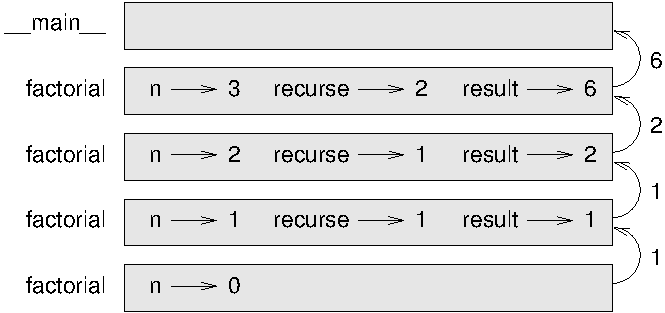
\includegraphics[scale=0.8]{../source/figs/stack3.pdf}}
\caption{堆栈图。}
\label{fig.stack3}
\end{figure}

%🍁% The return values are shown being passed back up the stack.  In each
%🍁% frame, the return value is the value of {\tt result}, which is the
%🍁% product of {\tt n} and {\tt recurse}.

图中的返回值被描绘为不断被传回到栈顶。 在每个栈帧中,返回值就是结果值,即是 \li{n} 和 \li{recurse} 的乘积。
\index{function frame}  \index{frame}

%🍁% In the last frame, the local variables {\tt recurse} and {\tt result} do not exist, because the branch that creates them does not run.

最后一帧中,局部变量 \li{recurse} 和 \li{result} 并不存在, 因为生成它们的分支并没有执行。


%🍁% \section{Leap of faith  |  信仰之跃}
\section{信仰之跃}
\index{recursion}  \index{leap of faith}

%🍁% Following the flow of execution is one way to read programs, but
%🍁% it can quickly become overwhelming.  An
%🍁% alternative is what I call the ``leap of faith''.  When you come to a
%🍁% function call, instead of following the flow of execution, you {\em
%🍁% assume} that the function works correctly and returns the right
%🍁% result.

跟随程序执行流程是阅读程序代码的一种方法,但它可能很快会变得错综复杂。
有另外一种替代方法,我称之为``信仰之跃''。
当你遇到一个函数调用时,不再去跟踪执行流程,而是 {\bf 假设} 这个函数正确运行并返回了正确的结果。

%🍁% In fact, you are already practicing this leap of faith when you use
%🍁% built-in functions.  When you call {\tt math.cos} or {\tt math.exp},
%🍁% you don't examine the bodies of those functions.  You just
%🍁% assume that they work because the people who wrote the built-in
%🍁% functions were good programmers.

事实上,当你使用内建函数时,你已经在实践这种方法了。
当你调用 \li{math.cos} 或 \li{math.exp} 时,你并没有检查那些函数的函数体。
你只是假设了它们能用,因为编写这些内建函数的人都是优秀的程序员。

%🍁% The same is true when you call one of your own functions.  For
%🍁% example, in Section~\ref{boolean}, we wrote a function called
%🍁% \verb"is_divisible" that determines whether one number is divisible by
%🍁% another.  Once we have convinced ourselves that this function is
%🍁% correct---by examining the code and testing---we can use the function
%🍁% without looking at the body again.

当你调用一个自己写的函数时也是一样。
例如,在 \ref{boolean} 节中,我们写了一个 \li{is_divisible} 函数来判断一个数能否被另一个数整除。
通过对代码的检查,一旦我们确信这个函数能够正确运行 --- 我们就能不用再查看函数体而直接使用了。
\index{testing!leap of faith}

%🍁% The same is true of recursive programs.  When you get to the recursive
%🍁% call, instead of following the flow of execution, you should assume
%🍁% that the recursive call works (returns the correct result) and then ask
%🍁% yourself, ``Assuming that I can find the factorial of $n-1$, can I
%🍁% compute the factorial of $n$?''  It is clear that you
%🍁% can, by multiplying by $n$.

递归程序也是这样。
当你遇到递归调用时, 不用顺着执行流程,你应该假设每次递归调用能够正确工作 (返回正确的结果), 然后问你自己,``假设我可以找到 $n-1$ 的阶乘,我可以找到 $n$ 的阶乘吗?''
很明显你能,只要再乘以 $n$ 即可。

%🍁% Of course, it's a bit strange to assume that the function works
%🍁% correctly when you haven't finished writing it, but that's why
%🍁% it's called a leap of faith!

当然,在你没写完函数的时就假设函数正确工作有一点儿奇怪, 但这也是为什么这被称作信仰之跃了!


%🍁% \section{One more example  |  再举一例}
\section{再举一例}
\label{one.more.example}

\index{fibonacci function}  \index{function!fibonacci}

%🍁% After {\tt factorial}, the most common example of a recursively
%🍁% defined mathematical function is {\tt fibonacci}, which has the
%🍁% following definition (see
  %🍁% \url{http://en.wikipedia.org/wiki/Fibonacci_number}):

除了阶乘以外,使用递归定义的最常见数学函数是 \li{fibonacci} (斐波那契数列),见其 \href{http://en.wikipedia.org/wiki/Fibonacci_number}{定义} :

\index{维基百科}

%
\begin{eqnarray*}
&& \mathrm{fibonacci}(0) = 0 \\
&& \mathrm{fibonacci}(1) = 1 \\
&& \mathrm{fibonacci}(n) = \mathrm{fibonacci}(n-1) + \mathrm{fibonacci}(n-2)
\end{eqnarray*}

%
%🍁% Translated into Python, it looks like this:

翻译成 Python ,看起来就像这样:

\begin{lstlisting}
def fibonacci (n):
    if n == 0:
        return 0
    elif  n == 1:
        return 1
    else:
        return fibonacci(n-1) + fibonacci(n-2)
\end{lstlisting}

%
%🍁% If you try to follow the flow of execution here, even for fairly
%🍁% small values of $n$, your head explodes.  But according to the
%🍁% leap of faith, if you assume that the two recursive calls
%🍁% work correctly, then it is clear that you get
%🍁% the right result by adding them together.

这里,如果你试图跟踪执行流程,即使是相当小的 $n$ ,也足够你头疼的。但遵循信仰之跃这种方法,如果你假设这两个递归调用都能正确运行,很明显将他们两个相加就是正确结果。

\index{flow of execution}


%🍁% \section{Checking types  |  检查类型}
\section{检查类型}
\label{guardian}

%🍁% What happens if we call {\tt factorial} and give it 1.5 as an argument?

如果我们将 1.5 作为参数调用阶乘函数 ( \li{factorial} )会怎样?

\index{type checking}  \index{error checking}
\index{factorial function}  \index{RuntimeError}

\begin{lstlisting}
>>> factorial(1.5)
RuntimeError: Maximum recursion depth exceeded
\end{lstlisting}

%
%🍁% It looks like an infinite recursion.  How can that be?  The function
%🍁% has a base case---when {\tt n == 0}.  But if {\tt n} is not an integer,
%🍁% we can {\em miss} the base case and recurse forever.

看上去像是一个无限循环。但那是如何发生的? 函数的基础情形是 \li{n == 0} 。
但是如果 \li{n} 不是一个整型数呢,我们会 {\em 错过} 基础情形,永远递归下去。
\index{infinite recursion}  \index{recursion!infinite}

%🍁% In the first recursive call, the value of {\tt n} is 0.5.
%🍁% In the next, it is -0.5.  From there, it gets smaller
%🍁% (more negative), but it will never be 0.

在第一次递归调用中,\li{n} 的值是 $0.5$ 。下一次,是 $-0.5$ 。自此它会越来越小,但永远不会是 $0$ 。

%🍁%  We have two choices.  We can try to generalize the {\tt factorial}
%🍁%  function to work with floating-point numbers, or we can make {\tt
  %🍁%  factorial} check the type of its argument.  The first option is
%🍁%  called the gamma function and it's a
%🍁%  little beyond the scope of this book.  So we'll go for the second.

我们有两个选择。我们可以试着泛化 \li{factorial} 函数,使其能处理浮点数,或者我们可以让 \li{factorial} 检查实参的类型。第一个选择被称作 \li{gamma} 函数,它有点儿超过本书的范围了。 所以我们将采用第二种方法。
\index{gamma function}
\index{gamma 函数}

%🍁% We can use the built-in function {\tt isinstance} to verify the type
%🍁% of the argument.  While we're at it, we can also make sure the
%🍁% argument is positive:

我们可以使用内建函数 \li{isinstance} 来验证实参的类型。 同时,我们也可以确保该实参是正数:
\index{isinstance function}  \index{function!isinstance}

\begin{lstlisting}
def factorial (n):
    if not isinstance(n, int):
        print('Factorial is only defined for integers.')
        return None
    elif n < 0:
        print('Factorial is not defined for negative integers.')
        return None
    elif n == 0:
        return 1
    else:
        return n * factorial(n-1)
\end{lstlisting}

%
%🍁% The first base case handles nonintegers; the
%🍁% second handles negative integers.  In both cases, the program prints
%🍁% an error message and returns {\tt None} to indicate that something
%🍁% went wrong:

第一个基础情形处理非整型数;第二个处理负整型数。
在这两个情形中,程序打印一条错误信息,并返回 \li{None} 以指明出现了错误:


\begin{lstlisting}
>>> factorial('fred')
Factorial is only defined for integers.
None
>>> factorial(-2)
Factorial is not defined for negative integers.
None
\end{lstlisting}

%
%🍁% If we get past both checks, we know that $n$ is positive or
%🍁% zero, so we can prove that the recursion terminates.

如果我们通过了这两个检查,那么我们知道 $n$ 是一个正数或 $0$ , 因此我们可以证明递归会终止。
\index{guardian pattern}  \index{pattern!guardian}

%🍁% This program demonstrates a pattern sometimes called a {\bf guardian}.
%🍁% The first two conditionals act as guardians, protecting the code that
%🍁% follows from values that might cause an error.  The guardians make it
%🍁% possible to prove the correctness of the code.

此程序演示了一个有时被称作 {\em 监护人} (guardian) 的模式。
前两个条件扮演监护人的角色,避免接下来的代码使用引发错误的值。
监护人使得验证代码的正确性成为可能。


%🍁% In Section~\ref{raise} we will see a more flexible alternative to printing
%🍁% an error message: raising an exception.

在\hyperref[raise]{反向查找} (Reverse Lookup) 一节中,我们将看到更灵活地打印错误信息的方式:抛出异常。

%🍁% \section{Debugging  |  调试}
\section{调试}
\label{factdebug}

%🍁% Breaking a large program into smaller functions creates natural
%🍁% checkpoints for debugging.  If a function is not
%🍁% working, there are three possibilities to consider:

将一个大程序分解为较小的函数为调试生成了自然的检查点。
如果一个函数不如预期的运行,有三个可能性需要考虑:

\index{debugging}

\begin{itemize}

%🍁% \item There is something wrong with the arguments the function
%🍁% is getting; a precondition is violated.

\item 该函数获得的实参有些问题,违反先决条件。

%🍁% \item There is something wrong with the function; a postcondition
%🍁% is violated.

\item 该函数有些问题,违反后置条件。

%🍁% \item There is something wrong with the return value or the
%🍁% way it is being used.

\item 返回值或者它的使用方法有问题。

\end{itemize}

%🍁% To rule out the first possibility, you can add a {\tt print} statement
%🍁% at the beginning of the function and display the values of the
%🍁% parameters (and maybe their types).  Or you can write code
%🍁% that checks the preconditions explicitly.

为了排除第一种可能,你可以在函数的开始增加一条 \li{print} 语句来打印形参的值(也可以是它们的类型)。
或者你可以写代码来显示地检查先决条件。
\index{precondition}  \index{postcondition}

%🍁% If the parameters look good, add a {\tt print} statement before each
%🍁% {\tt return} statement and display the return value.  If
%🍁% possible, check the result by hand.  Consider calling the
%🍁% function with values that make it easy to check the result
%🍁% (as in Section~\ref{incremental.development}).

如果形参看起来没问题,就在每个 \li{return} 语句之前增加一条 \li{print} 语句,来打印返回值。
如果可能,手工检查结果。
考虑用一些容易检查的值来调用该函数(类似在 \hyperref[incremental.development]{小节} 中那样)。


%🍁% If the function seems to be working, look at the function call
%🍁% to make sure the return value is being used correctly (or used
%🍁% at all!).

如果该函数看起来正常工作,则检查函数调用,确保返回值被正确的使用(或者的确被使用了!)。
\index{flow of execution}

%🍁% Adding print statements at the beginning and end of a function
%🍁% can help make the flow of execution more visible.
%🍁% For example, here is a version of {\tt factorial} with
%🍁% print statements:

在一个函数的开始和结尾处增加打印语句,可以使执行流程更明显。
例如,下面是一个带打印语句的阶乘函数:

\begin{lstlisting}
def factorial(n):
    space = ' ' * (4 * n)
    print(space, 'factorial', n)
    if n == 0:
        print(space, 'returning 1')
        return 1
    else:
        recurse = factorial(n-1)
        result = n * recurse
        print(space, 'returning', result)
        return result
\end{lstlisting}

%
%🍁% {\tt space} is a string of space characters that controls the
%🍁% indentation of the output.  Here is the result of {\tt factorial(4)} :

\li{space} 是一个空格字符的字符串,用来控制输出的缩进。 下面是 \li{factorial(4)} 的输出结果:


\begin{lstlisting}
                 factorial 4
             factorial 3
         factorial 2
     factorial 1
 factorial 0
 returning 1
     returning 1
         returning 2
             returning 6
                 returning 24
\end{lstlisting}

%
%🍁% If you are confused about the flow of execution, this kind of
%🍁% output can be helpful.  It takes some time to develop effective
%🍁% scaffolding, but a little bit of scaffolding can save a lot of debugging.

如果你对执行流程感到困惑,这种输出可能有助于理解。
开发有效的脚手架代码会花些时间,但是一点点的脚手架代码能够节省很多的调试时间。

%🍁% \section{Glossary  |  术语表}
\section{术语表}

\begin{description}

%🍁% \item[temporary variable:]  A variable used to store an intermediate value in
%🍁% a complex calculation.
\index{temporary variable}  \index{variable!temporary}
\index{临时变量}  \index{变量!临时}

\item[临时变量 (temporary variable):] 一个在复杂计算中用于存储过度值的变量。

%🍁% \item[dead code:]  Part of a program that can never run, often because
%🍁% it appears after a {\tt return} statement.
\index{dead code}
\index{死代码}

\item[死代码 (dead code):] 程序中永远无法执行的那部分代码,通常是因为其出现在一个返回语句之后。

%🍁% \item[incremental development:]  A program development plan intended to
%🍁% avoid debugging by adding and testing only
%🍁% a small amount of code at a time.
\index{incremental development}
\index{增量式开发}

\item[增量式开发 (incremental development):] 一种程序开发计划,目的是通过一次增加及测试少量代码的方式,来避免长时间的调试。

%🍁% \item[scaffolding:]  Code that is used during program development but is
%🍁% not part of the final version.
\index{scaffolding}
\index{脚手架代码}

\item[脚手架代码 (scaffolding):] 程序开发中使用的代码,但并不是最终版本的一部分。

%🍁% \item[guardian:]  A programming pattern that uses a conditional
%🍁% statement to check for and handle circumstances that
%🍁% might cause an error.
\index{guardian pattern}  \index{pattern!guardian}
\index{监护人模式}  \index{模式!监护人}

\item[监护人 (guardian):] 一种编程模式,使用条件语句来检查并处理可能引发错误的情形。

\end{description}


%🍁% \section{Exercises  |  练习}
\section{练习}

\begin{exercise}

%🍁% Draw a stack diagram for the following program.  What does the program print?

画出下面程序的堆栈图。
这个程序的最终输出是什么?
\index{stack diagram}  \index{堆栈图}

\begin{em}
\begin{lstlisting}
def b(z):
    prod = a(z, z)
    print(z, prod)
    return prod

def a(x, y):
    x = x + 1
    return x * y

def c(x, y, z):
    total = x + y + z
    square = b(total)**2
    return square

x = 1
y = x + 1
print(c(x, y+3, x+y))
\end{lstlisting}
\end{em}

\end{exercise}


\begin{exercise}
\label{ackermann}

%🍁% The Ackermann function, $A(m, n)$, is defined:

{\em Ackermann} 函数 $A(m, n)$ 的定义如下:

\begin{eqnarray*}
A(m, n) = \begin{cases}
              n+1 & \mbox{if } m = 0 \\
        A(m-1, 1) & \mbox{if } m > 0 \mbox{ and } n = 0 \\
A(m-1, A(m, n-1)) & \mbox{if } m > 0 \mbox{ and } n > 0.
\end{cases}
\end{eqnarray*}

%
%🍁% See \url{http://en.wikipedia.org/wiki/Ackermann_function}.
%🍁% Write a function named {\tt ack} that evaluates the Ackermann function.
%🍁% Use your function to evaluate {\tt ack(3, 4)}, which should be 125.
%🍁% What happens for larger values of {\tt m} and {\tt n}?
%🍁% Solution: \url{http://thinkpython2.com/code/ackermann.py}.

查看 \href{http://en.wikipedia.org/wiki/Ackermann_function}{维基百科的定义},
编写一个叫作 {\em \li{ack}} 的函数来计算 {\em Ackermann} 函数。
使用你的函数计算 {\em \li{ack(3,4)}},其结果应该为 $125$ 。
如果 {\em \li{m}} 和 {\em \li{n}} 的值较大时,会发生什么?
\href{http://thinkpython2.com/code/ackermann.py}{参考答案}

\index{Ackermann function}  \index{function!ack}
\index{阿克曼函数}  \index{函数!阿克曼}
\index{维基百科}
\end{exercise}


\begin{exercise}
\label{palindrome}

%🍁% A palindrome is a word that is spelled the same backward and
%🍁% forward, like ``noon'' and ``redivider''.  Recursively, a word
%🍁% is a palindrome if the first and last letters are the same
%🍁% and the middle is a palindrome.

回文词 {\em (palindrome)} 指的是正着拼反着拼都一样的单词,如 {\em ``noon''} 和 {\em ``redivider''}。
按照递归定义的话, 如果某个词的首字母和尾字母相同, 而且中间部分也是一个回文词, 那它就是一个回文词。
\index{palindrome}

%🍁% The following are functions that take a string argument and
%🍁% return the first, last, and middle letters:

下面的函数接受一个字符串实参,并返回第一个、最后一个和中间的字母:

\begin{em}
\begin{lstlisting}
def first(word):
    return word[0]

def last(word):
    return word[-1]

def middle(word):
    return word[1:-1]
\end{lstlisting}
\end{em}

%
%🍁% We'll see how they work in Chapter~\ref{strings}.

在 \hyperref[strings]{第八章} 中我们将介绍它们是如何工作的。

%🍁% \begin{enumerate}
%🍁%
%🍁% \item Type these functions into a file named {\tt palindrome.py}
%🍁% and test them out.  What happens if you call {\tt middle} with
%🍁% a string with two letters?  One letter?  What about the empty
%🍁% string, which is written \verb"''" and contains no letters?
%🍁%
%🍁% \item Write a function called \verb"is_palindrome" that takes
%🍁% a string argument and returns {\tt True} if it is a palindrome
%🍁% and {\tt False} otherwise.  Remember that you can use the
%🍁% built-in function {\tt len} to check the length of a string.
%🍁%
%🍁% \end{enumerate}

\begin{enumerate}

\item 将它们录入到文件 {\em \li{palindrome.py}} 中并测试。当你用一个两个字母的字符串调用 {\em \li{middle}} 时会发生什么?一个字母的呢?空字符串呢?空字符串这样 {\em \li{"''"}} 表示,中间不含任何字母。

\item 编写一个叫 {\em \li{is_palindrome}} 的函数, 接受一个字符串作为实参。 如果是回文词, 就返回 {\em \li{True}} ,反之则返回 {\em \li{False}} 。记住, 你可以使用内建函数 {\em \li{len}} 来检查字符串的长度。

\end{enumerate}

%🍁% Solution: \url{http://thinkpython2.com/code/palindrome_soln.py}.

\href{http://thinkpython2.com/code/palindrome_soln.py}{参考答案}

\end{exercise}

\begin{exercise}

%🍁% A number, $a$, is a power of $b$ if it is divisible by $b$
%🍁% and $a/b$ is a power of $b$.  Write a function called
%🍁% \verb"is_power" that takes parameters {\tt a} and {\tt b}
%🍁% and returns {\tt True} if {\tt a} is a power of {\tt b}.
%🍁% Note: you will have to think about the base case.

当数字 $a$ 能被  $b$ 整除,并且 $a/b$ 是 $b$ 的幂时, 它就是 $b$ 的幂。
编写一个叫 {\em \li{is_power}} 的函数,接受两个参数 {\em \li{a}} 和 {\em \li{b}}, 并且当 {\em \li{a}} 是 {\em \li{b}} 的幂时返回 {\em \li{True}}。
注意:你必须要想好基础情形。

\end{exercise}

\begin{exercise}
\index{greatest common divisor (GCD)}  \index{GCD (greatest common divisor)}

%🍁% The greatest common divisor (GCD) of $a$ and $b$ is the largest number
%🍁% that divides both of them with no remainder.

$a$ 和 $b$ 的最大公约数 {\em (reatest common divisor, GCD)}是能被二者整除的最大数。

%🍁% One way to find the GCD of two numbers is based on the observation
%🍁% that if $r$ is the remainder when $a$ is divided by $b$, then $gcd(a,
%🍁% b) = gcd(b, r)$.  As a base case, we can use $gcd(a, 0) = a$.

求两个数的最大公约数的一种方法,是基于这样一个原理:如果 $r$ 是 $a$ 被 $b$ 除后的余数,那么  $gcd(a,b) = gcd(b, r)$ 。我们可以把 $gcd(a, 0) = a$ 当做基础情形。

%🍁% Write a function called
%🍁% \verb"gcd" that takes parameters {\tt a} and {\tt b}
%🍁% and returns their greatest common divisor.

编写一个叫 {\em \li{gcd}} 的函数,接受两个参数 {\em \li{a}} 和 {\em \li{b}},并返回二者的最大公约数。

%🍁% Credit: This exercise is based on an example from Abelson and
%🍁% Sussman's {\em Structure and Interpretation of Computer Programs}.

致谢:这道习题基于 {\em Abelson} 和 {\em Sussman} 编写的 《Structure and Interpretation of Computer Programs》 中的例子。

\end{exercise}
